\section{Návrh metód s MaFaulDa}
Súbor údajov MaFaulDa používame ako smerodajný pri určovaní metód schopných nasadenia na senzorovú jednotku. MaFaulda obsahuje 1951 záznamov so vzorkovaciu frekvenciu 50 kHz a označenými simulovanými poruchami rôznej závažnosti. Nahrávky obsahujú časové rady z dvoch trojosích piezoelektrických akcelerometrov. Po úprave ponechávame 6 typov značiek: referenčný bezporuchový stav, dve poruchy hriadeľa (nevyváženosť, nesúososť) a tri poruchy ložísk (poruchy klietky, guľôčok, vonkajšieho krúžku). 

Zo signálov rozdeleních na päť jednosekundových častí sa odstraňuje jednosmerná zložka odčítaním priemernej akcelerácie, po ktorej nasleduje dolnopriepustný 10 kHz filter. Z častí signálu je potom vytvorených 10 časových a 11 spektrálnych premenných. Euklidovská norma trojrozmerných atribútov eliminuje závislosť na smere merania. Pri výbere atribútov nie je do množiny pridaná taká dvojica, ak ich absolútna hodnota korelácie presahuje 0.95.

Predpokladáme, že dátové body rozprestreté v každej dimenzii priestoru môžu dobre rozlíšiť skupiny. Ukazuje sa, že premenné sú navzájom viac korelované v časovej doméne ako ilustruje analýza hlavných komponentov. Pre 95\% vysvetleného rozptylu PCA sú v časovej doméne potrebné 3 zložky, zatiaľ čo vo frekvenčnej doméne 4 zložky. PCA efektívne vyjadruje atribúty v menej rozmernom priestore, ale ich výslednou lineárnou kombináciou sa ťažko odôvodňujú rozhodnutia modelu.

Pri posudzovaní všeobecne najdôležitejších atribútov vychádzame z trojíc nekorelovaných atribútov vytvorených v 24 scenároch. Podmienky scenárov vznikli kombináciou štyroch kritérií: dávkové alebo inkrementálne učenie, pozícia ložiska, predikovaná premenná, limit na rotačnú rýchlosť. Na základe schvaľovacieho hlasovania sú najčastejšie sa vyskytujúcimi atribútmi v časovej doméne: špička-špička, faktor tvaru, faktor výkyvu. Vo frekvenčnej doméne sú to spektrálne ťažisko, roll-on a roll-off.

Tri typy experimentov s modelom k-NN prebiehajú s validáciou metódou hold-out, Najprv sa model naučí všetky extrahované prvky, takže nedochádza k výberu prvkov. Metódou hrubej sily sa hľadá kombinácia troch atribútov s najvyššou trénovaciou presnosťou. Následne sa porovnáva presnosť modelu pre tri atribúty zvolené technikami výberu atribútov. Dávkový model k-NN slúži ako referenčný, podľa ktorého sa posudzuje k-NN v postupnom učení.

Online učenie napodobňuje sťažené podmienky diagnostiky strojov, ktoré sa objavujú v praxi. Oneskorené dodanie alebo vynechanie skutočných značiek nepochybne znižuje spoľahlivosť klasifikácie. Modely k-NN v experimentoch s postupným učením sú trénované na rovnakom základnom súbore údajov pre ložisko A nad všetkými extrahovanými atribútmi. Týmto spôsobom môžeme porovnať trénovacie presnosti tréningu pre dávkové a postupné učenie. k-NN sme nastavili na 5 susedov a euklidovskú vzdialenosť. Metriky online učenia sa vyhodnocujú v metódou progresívnom vyhodnocovanie na ešte nevyváženom súbore údajov.

\section{Zber vibrácií v priemysle}
Doteraz uplatnená metodika pre súbor údajov zaznamenaných v laboratóriu sa aplikuje na vibračných signáloch z priemyselného prostredia. Pri monitorovaní zužitkujeme mierne prispôsobený postup z noriem. Ten zahŕňa výber strojov určených na monitorovanie, identifikáciu pozícií na meranie podľa technických štandardov, predbežné merania a vývoj senzorovej jednotky. Zber nového súboru údajov sprevádza vopred dohodnutý harmonogram.

Na zber údajov boli vyčlenené dva špirálové kompresory ako súčasť klimatizačných jednotiek pre dátové centrum a tri čerpadlá s troma elektrometrami v prečerpávacej stanici na pitnú vodu. Dlhodobejšie merania uskutočníme vlastným vnoreným systémom na báze vývojovej dosky ESP32-PoE-ISO so slotom na SD kartu. Ako senzor vibrácii použijeme MEMS akcelerometer IIS3DWB. Vyznačuje sa vysokou šírkou pásma až 6.3 kHz, nízkym šumom, a vysokou výstupným dátovým tokom 26.7 kHz cez SPI zbernicu.

\section{Záver}
V diplomovej práci sme sa zamerali na výber trendových ukazovateľov pre riešenie monitorovania prevádzkového stavu a odhaľovanie porúch z vibračných signálov.  Extrahované premenné pochádzajú hlavne z popisných štatistík, z článkov o spracovaní zvukových signálov a technických noriem vibrodiagnostiky.

Dosiahnuté stratové kompresné pomery pre MaFaulDa sú 2381:1 pre všetky atribúty a 25000:1 pre šesť atribútov. Výber atribútov metódou súčinu poradí zabezpečí väčšinou najlepšiu presnosť k-NN modelu oproti metrikám samostatne. Žiadny prístup však nedokázal nájsť trojicu prediktorov s presnosťou blízkou optimálnej, ktorá je až 98\%. Trénovanie k-NN na troch hlavných komponentoch prinieslo lepšiu presnosť ako výber atribútov. 

Model postupného učenia k-NN dosahuje prinajlepšom 90\% presnosť s okamžitou spätnou väzbou, 85\% so značkami oneskorenými o 250 pozorovaní a 82\% s iba 25\% anotovaného súboru údajov. Porovnateľný model trénovaný v dávkach dosahuje presnosť 98\%.  Doteraz boli urobené závery podľa súboru údajov MaFaulDa, ktoré plánujeme overiť na súbore údajov získaných v priemysle počas DP3.

% Features range (3D)
% Standing Fan
\begin{figure}[h]
    \centering
    \begin{subfigure}[b]{0.48\textwidth}
        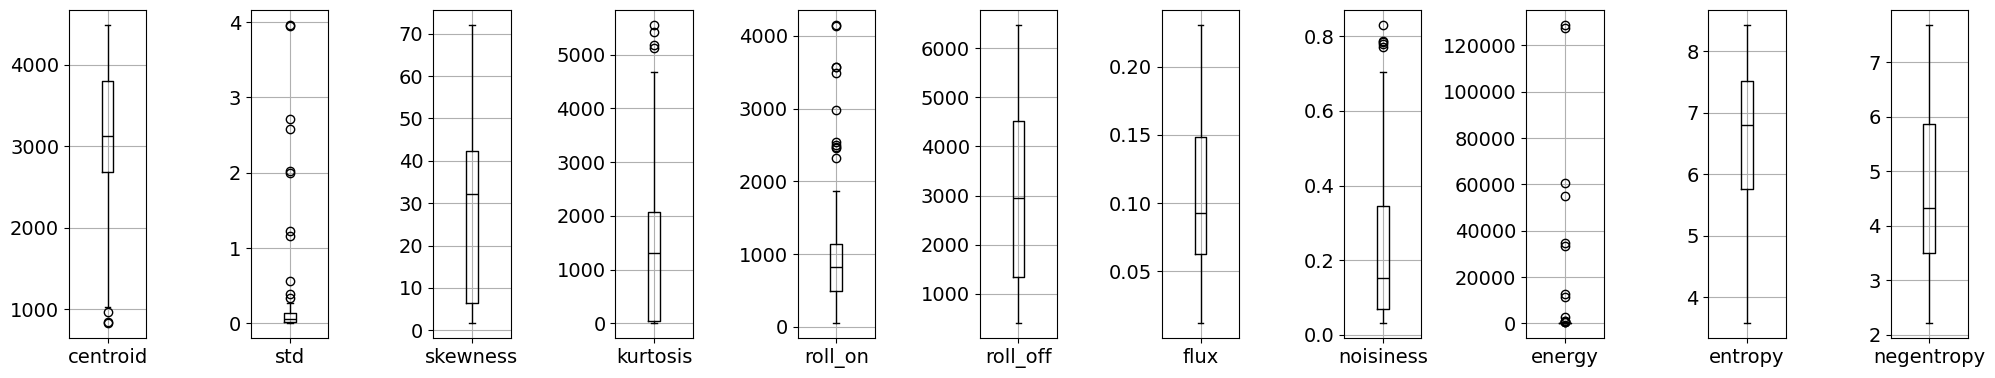
\includegraphics[width=\textwidth]{assets/results/feature-values/fan-TD-features.png}
        \caption{Time-domain features}
    \end{subfigure}
    \hfill
    \begin{subfigure}[b]{0.48\textwidth}
        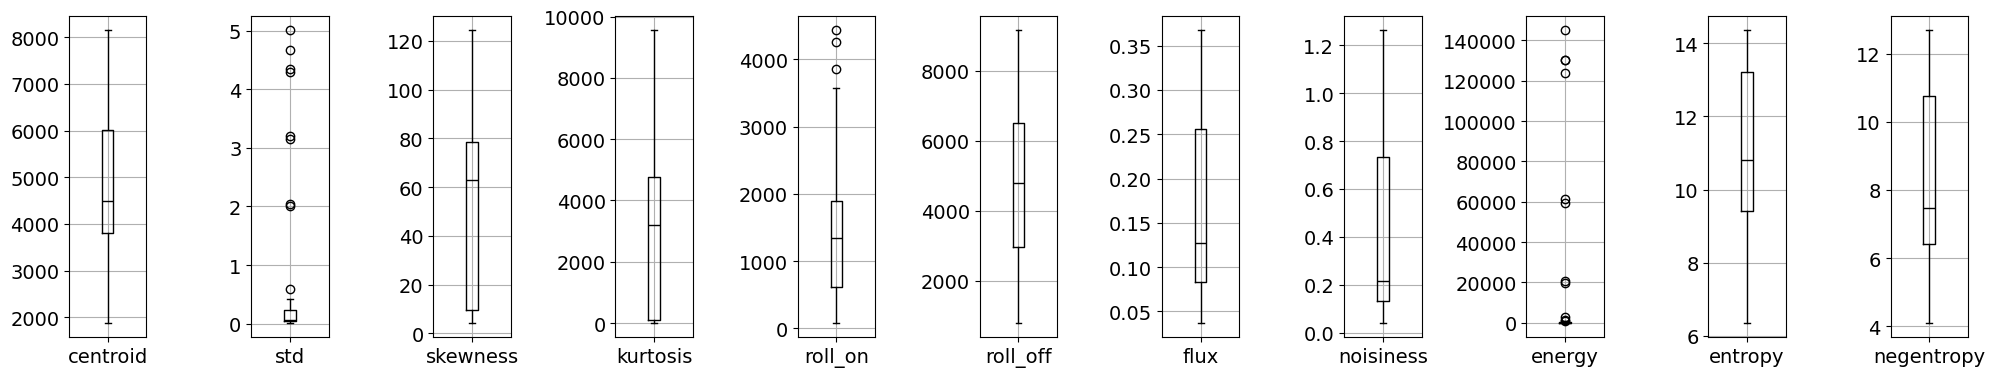
\includegraphics[width=\textwidth]{assets/results/feature-values/fan-FD-features.png}
        \caption{Frequency-domain features}
    \end{subfigure}
    \caption{Feature range in standing fan}
\end{figure}
